% -*- TeX -*- -*- UK -*- -*- Soft -*-

\chapter{Understanding Bayes}
\label{chap:UnderstandingBayes}


Taken verbatim from \cite{etz2015a,etz2015d,etz2015b,etz2015c,etz2016a}.
All these blog posts have lively discussion, please see the web sites.

\section{A Look at the Likelihood}
\label{sec:ALookattheLikelihood}

Much of the discussion in psychology surrounding Bayesian inference focuses on priors. Should we embrace priors, or should we be skeptical? When are Bayesian methods sensitive to specification of the prior, and when do the data effectively overwhelm it? Should we use context specific prior distributions or should we use general defaults? These are all great questions and great discussions to be having.

One thing that often gets left out of the discussion is the importance of the likelihood. The likelihood is the workhorse of Bayesian inference. In order to understand Bayesian parameter estimation you need to understand the likelihood. In order to understand Bayesian model comparison (Bayes factors) you need to understand the likelihood and likelihood ratios.

\subsection{What is likelihood?}

Likelihood is a funny concept. It's not a probability, but it is \textit{proportional} to a probability. The likelihood of a hypothesis ($H$) given some data ($D$) is proportional to the probability of obtaining $D$ given that $H$ is true, multiplied by an arbitrary positive constant ($K$). In other words, $\mathrm{L}(\mathrm{H} | \mathrm{D})=\mathrm{K} \cdot \mathrm{P}(\mathrm{D} | \mathrm{H})$. Since a likelihood isn't actually a probability it doesn't obey various rules of probability. For example, likelihood need not sum to 1.

A critical difference between probability and likelihood is in the interpretation of what is fixed and what can vary. In the case of a conditional probability, $\mathrm{P}(\mathrm{D} | \mathrm{H})$, the hypothesis is fixed and the data are free to vary. Likelihood, however, is the opposite. The likelihood of a hypothesis, $\mathrm{L}(\mathrm{H} | \mathrm{D})$, conditions on the data as if they are fixed while allowing the hypotheses to vary.

The distinction is subtle, so I'll say it again. For conditional probability, the hypothesis is treated as a given and the data are free to vary. For likelihood, the data are a given and the hypotheses vary.
The Likelihood Axiom

Edwards \cite[p 30]{Edwards1992} defines the Likelihood Axiom as a natural combination of the Law of Likelihood and the Likelihood Principle.

The \textbf{Law of Likelihood} states that ``within the framework of a statistical model, a particular set of data supports one statistical hypothesis better than another if the likelihood of the first hypothesis, on the data, exceeds the likelihood of the second hypothesis'' (Emphasis original, \cite[p 30]{Edwards1992}).

In other words, there is evidence for $H1$ vis-a-vis $H2$ if and only if the probability of the data under $H1$ is greater than the probability of the data under $H2$. That is, $D$ is evidence for $H1$ over $H2$ if $\mathrm{P}(\mathrm{D} | \mathrm{H} 1)>\mathrm{P}(\mathrm{D} | \mathrm{H} 2)$. If these two probabilities are equivalent, then there is no evidence for either hypothesis over the other. Furthermore, the strength of the statistical evidence for $H1$ over $H2$ is quantified by the ratio of their likelihoods, $\mathrm{L}(\mathrm{H} 1 | \mathrm{D}) / \mathrm{L}(\mathrm{H} 2 | \mathrm{D})$ (which again is proportional to $\mathrm{P}(\mathrm{D} | \mathrm{H} 1) / \mathrm{P}(\mathrm{D} | \mathrm{H} 2)$ up to an arbitrary constant that cancels out).

The \textbf{Likelihood Principle} states that the likelihood function contains all of the information relevant to the evaluation of statistical evidence. Other facets of the data that do not factor into the likelihood function are \textit{irrelevant} to the evaluation of the strength of the statistical evidence 
\cite[p 30]{Edwards1992},cite[p 22]{Royall2000}. They can be meaningful for planning studies or for decision analysis, but they are separate from the 
\textit{strength} of the statistical evidence.

\subsection{Likelihoods are meaningless in isolation}

Unlike a probability, a likelihood has no real meaning \textit{per se} due to the arbitrary constant. Only by comparing likelihoods do they become interpretable, because the constant in each likelihood cancels the other one out. The easiest way to explain this aspect of likelihood is to use the binomial distribution as an example.

Suppose I flip a coin 10 times and it comes up 6 heads and 4 tails. If the coin were fair, p(heads) = .5, the probability of this occurrence is defined by the binomial distribution:
\begin{equation}
P(X=x)=
\left(\begin{array}{l}
n \\x\end{array}\right) 
p^{x}(1-p)^{n-x}
\end{equation}
where $x$ is the number of heads obtained, $n$ is the total number of flips, $p$ is the probability of heads, and
\begin{equation}
\left(\begin{array}{l}
n \\x\end{array}\right)
=\frac{n !}{x !(n-x) !}
\end{equation}
Substituting in our values we get
\begin{equation}P(X=6)=\frac{10 !}{6 !(4 !)}(.5)^{6}(1-.5)^{4} \approx .21\end{equation}
If the coin were a trick coin, so that p(heads) = .75, the probability of 6 heads in 10 tosses is:
\begin{equation}P(X=6)=\frac{10 !}{6(4 ! !)}(.75)^{6}(1-.75)^{4} \approx .15\end{equation}
To quantify the statistical evidence for the first hypothesis against the second, we simply divide one probability by the other. This ratio tells us everything we need to know about the support the data lends to one hypothesis vis-a-vis the other.  In the case of 6 heads in 10 tosses, the likelihood ratio (LR) for a fair coin vs our trick coin is:
\begin{equation}L R=\left(\frac{10 !}{6 !(4 !)}(.5)^{6}(1-.5)^{4}\right) \div\left(\frac{10 !}{6 !(4 !)}(.75)^{6}(1-.75)^{4}\right) \approx .21 / .15 \approx 1.4\end{equation}
Translation: The data are 1.4 times as probable under a fair coin hypothesis than under this particular trick coin hypothesis. Notice how the first terms in each of the equations above, i.e., $\frac{10 !}{6 !(4 !)}$ , are equivalent and completely cancel each other out in the likelihood ratio.

\textsl{Same data. Same constant. Cancel out.}

The first term in the equations above, $\frac{10 !}{6 !(4 !)}$, details \textit{our journey} to obtaining 6 heads out of 10. If we change our journey (i.e., different sampling plan) then this changes the term's value, \textbf{but crucially, since it is the same term in both the numerator and denominator it always cancels itself out}. In other words, the information contained in the way the data are obtained \textit{disappears from the function}. Hence the irrelevance of the stopping rule to the evaluation of statistical evidence, which is something that makes Bayesian and likelihood methods valuable and flexible.

If we leave out the first term in the above calculations, our numerator is $L(.5)=0.0009765625$
 and our denominator is $\mathrm{L}(.75) \approx 0.0006952286$. Using these values to form the likelihood ratio we get: $0.0009765625 / 0.0006952286 \approx 1.4$, as we should since the other terms simply cancelled out before.

Again I want to reiterate that the value of a single likelihood is meaningless in isolation; only in \textit{comparing} likelihoods do we find meaning.

\subsection{Looking at likelihoods}

Likelihoods may seem overly restrictive at first. We can only compare 2 simple statistical hypotheses in a single likelihood ratio. But what if we are interested in comparing many more hypotheses at once? What if we want to compare all possible hypotheses at once?

In that case we can plot the likelihood function for our data, and this lets us ‘see' the evidence in its entirety. By plotting the entire likelihood function we compare all possible hypotheses simultaneously. The Likelihood Principle tells us that the likelihood function encompasses all statistical evidence that our data can provide, so we should always plot this function along side our reported likelihood ratios.

Following the wisdom of Birnbaum \cite{Birnbaum1962}, ``the ``evidential meaning'' of experimental results is characterized fully by the likelihood function'' (as cited in \cite[p 25]{Royall2000}). So let's look at some examples. The R script at the end of this post can be used to reproduce these plots, or you can use it to make your own plots. Play around with it and see how the functions change for different number of heads, total flips, and hypotheses of interest. See the instructions in the script for details.

The graph shows the likelihood function for 6 heads in 10 tosses. I've marked our two hypotheses from before on the likelihood curve with blue dots. Since the likelihood function is meaningful only up to an arbitrary constant, the graph is scaled by convention so that the best supported value (i.e., the maximum) corresponds to a likelihood of 1.

\begin{figure}[h]
    \centering
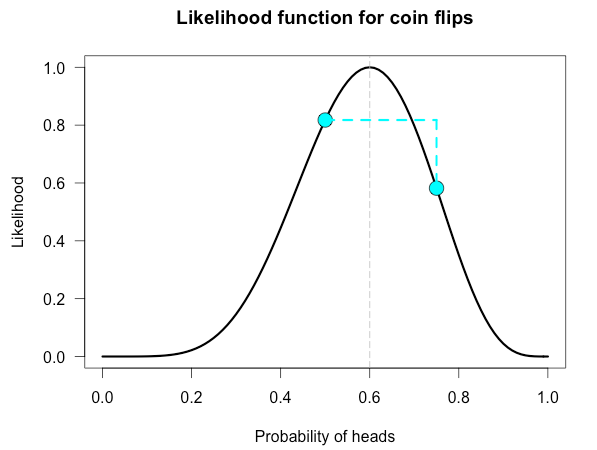
\includegraphics[width=0.8\textwidth]{pic/p05c03-snip01.png}
    \caption{Likelihood function for 6 heads in 10 flips}
    \label{fig:p05c03-snip01}
\end{figure}

The vertical dotted line marks the hypothesis best supported by the data. The likelihood ratio of any two hypotheses is simply the ratio of their heights on this curve. We can see from the plot that the fair coin has a higher likelihood than our trick coin.

How does the curve change if instead of 6 heads out of 10 tosses, we tossed 100 times and obtained 60 heads?

\begin{figure}[h]
    \centering
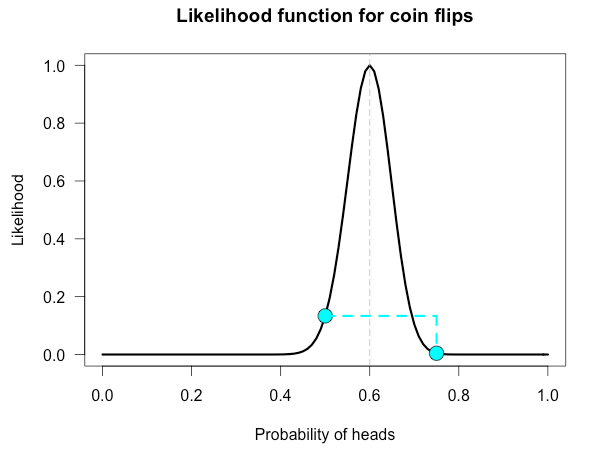
\includegraphics[width=.8\textwidth]{pic/p05c03-snip02.png}
    \caption{Likelihood function for  60 heads in 100  flips}
    \label{fig:p05c03-snip02}
\end{figure}

Our curve gets much narrower! How did the strength of evidence change for the fair coin vs the trick coin? The new likelihood ratio is $\mathrm{L}(.5) / \mathrm{L}(.75) \approx 29.9$. Much stronger evidence!\footnote{Obtaining 60 heads in 100 tosses is equivalent to obtaining 6 heads in 10 tosses 10 separate times. To obtain this new likelihood ratio we can simply multiply our ratios together. That is, raise the first ratio to the power of 10; $1.4^{\wedge} 10 \approx 28.9$, which is just slightly off from the correct value of 29.9 due to rounding.} However, due to the narrowing, neither of these hypothesized values are very high up on the curve anymore. It might be more informative to compare each of our hypotheses against the best supported hypothesis. This gives us two likelihood ratios: $\mathrm{L}(.6) / \mathrm{L}(.5) \approx 7.5$  and $\mathrm{L}(.6) / \mathrm{L}(.75) \approx 224$.

\begin{figure}[h]
    \centering
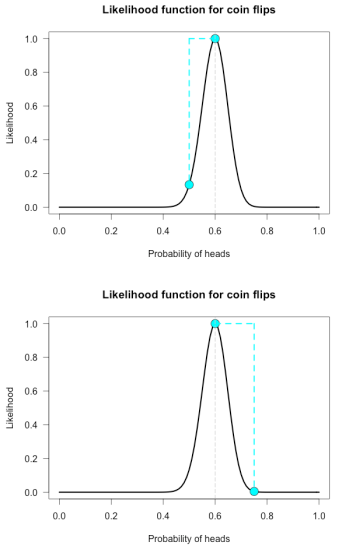
\includegraphics[width=0.8\textwidth]{pic/p05c03-snip03.png}
    \caption{Likelihood function ratios 7.5 and 224}
    \label{fig:p05c03-snip03}
\end{figure}

Here is one more curve, for when we obtain 300 heads in 500 coin flips.

\begin{figure}[h]
    \centering
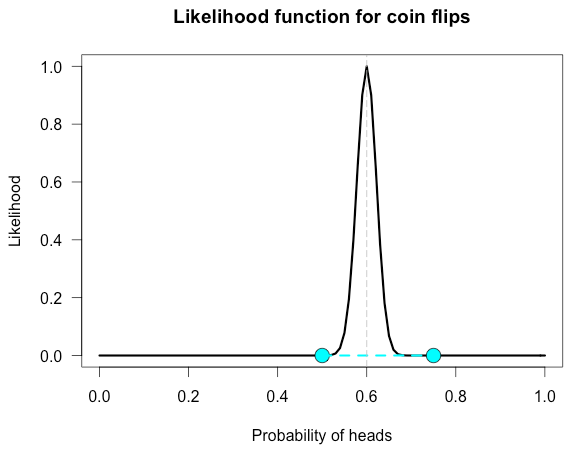
\includegraphics[width=0.8\textwidth]{pic/p05c03-snip04.png}
    \caption{Likelihood function for  300 heads in 500  flips}
    \label{fig:p05c03-snip04}
\end{figure}

Notice that both of our hypotheses look to be very near the minimum of the graph. Yet their likelihood ratio is much stronger than before. For this data the likelihood ratio$\mathrm{L}(.5) / \mathrm{L}(.75)$ is nearly \textbf{24 million!} The inherent relativity of evidence is made clear here: The fair coin was supported when compared to \textit{one particular} trick coin. But this should not be interpreted as absolute evidence for the fair coin, because the likelihood ratio for the maximally supported hypothesis vs the fair coin, $\mathrm{L}(.6) / \mathrm{L}(.5)$, is nearly \textbf{24 thousand!}

We need to be careful not to make blanket statements about absolute support, such as claiming that the maximum is ``strongly supported by the data''. Always ask, ``Compared to what?'' The best supported hypothesis will be only be weakly supported vs any hypothesis just before or just after it on the x-axis. For example, $\mathrm{L}(.6) / \mathrm{L}(.61) \approx 1.1$, which is barely any support one way or the other. It cannot be said enough that evidence for a hypothesis must be evaluated in consideration with a specific alternative.

\subsection{Connecting likelihood ratios to Bayes factors}

Bayes factors are simple extensions of likelihood ratios. A Bayes factor is a weighted average likelihood ratio based on the prior distribution specified for the hypotheses. (When the hypotheses are simple point hypotheses, the Bayes factor is equivalent to the likelihood ratio.) The likelihood ratio is evaluated at each point of the prior distribution and weighted by the probability we assign that value. If the prior distribution assigns the majority of its probability to values far away from the observed data, then the average likelihood for that hypothesis is lower than one that assigns probability closer to the observed data. In other words, you get a Bayes boost if you make more accurate predictions. Bayes factors are extremely valuable, and in a future post I will tackle the hard problem of assigning priors and evaluating weighted likelihoods.

I hope you come away from this post with a greater knowledge of, and appreciation for, likelihoods. Play around with the R code and you can get a feel for how the likelihood functions change for different data and different hypotheses of interest.


\begin{lstlisting}
## R code for the plots
## Plots the likelihood function for the data obtained
## h = number of successes (heads), n = number of trials (flips), 
## p1 = prob of success (head) on H1, p2 = prob of success (head) on H2
## Returns the likelihood ratio for p1 over p2. The default values are the ones used in the blog post
LR <- function(h,n,p1=.5,p2=.75){
        L1 <- dbinom(h,n,p1)/dbinom(h,n,h/n) ## Likelihood for p1, standardized vs the MLE
        L2 <- dbinom(h,n,p2)/dbinom(h,n,h/n) ## Likelihood for p2, standardized vs the MLE
        Ratio <- dbinom(h,n,p1)/dbinom(h,n,p2) ## Likelihood ratio for p1 vs p2
        curve((dbinom(h,n,x)/max(dbinom(h,n,x))), xlim = c(0,1), ylab = "Likelihood",xlab = "Probability of heads",las=1,
                main = "Likelihood function for coin flips", lwd = 3)
        points(p1, L1, cex = 2, pch = 21, bg = "cyan")
        points(p2, L2, cex = 2, pch = 21, bg = "cyan")
        lines(c(p1, p2), c(L1, L1), lwd = 3, lty = 2, col = "cyan")
        lines(c(p2, p2), c(L1, L2), lwd = 3, lty = 2, col = "cyan")
        abline(v = h/n, lty = 5, lwd = 1, col = "grey73")
        return(Ratio) ## Returns the likelihood ratio for p1 vs p2
}
\end{lstlisting}

Obtaining 60 heads in 100 tosses is equivalent to obtaining 6 heads in 10 tosses 10 separate times. To obtain this new likelihood ratio we can simply multiply our ratios together. That is, raise the first ratio to the power of 10; $1.4^{\wedge} 10 \approx 28.9$, which is just slightly off from the correct value of 29.9 due to rounding.

In the comments to the above blog, someone wrote:
`` Bayesian statistics is a religion that gives a false promise of certainty to believers in a world of uncertainty.''



\section{Updating priors via the likelihood}
\label{sec:Updatingpriorsviathelikelihood}

Above I outlined the basic idea behind likelihoods and likelihood ratios. Likelihoods are relatively straightforward to understand because they are based on tangible data. Collect your data, and then the likelihood curve shows the relative support that your data lend to various simple hypotheses. Likelihoods are a key component of Bayesian inference because they are the bridge that gets us from prior to posterior.

In this post I explain how to use the likelihood to update a prior into a posterior. The simplest way to illustrate likelihoods as an updating factor is to use \textit{conjugate distribution families} \cite{Raiffa2000}. A prior and likelihood are said to be conjugate when the resulting posterior distribution is the same type of distribution as the prior. This means that if you have binomial data you can use a beta prior to obtain a beta posterior. If you had normal data you could use a normal prior and obtain a normal posterior. Conjugate priors are not required for doing Bayesian updating, but they make the calculations a lot easier so they are nice to use if you can.

I'll use some data from a recent NCAA 3-point shooting contest to illustrate how different priors can converge into highly similar posteriors.

\subsection{The data}

This year's NCAA shooting contest was a thriller that saw Cassandra Brown of the Portland Pilots win the grand prize. This means that she won the women's contest and went on to defeat the men's champion in a shoot-off. This got me thinking, just how good is Cassandra Brown?

What a great chance to use some real data in a toy example. She completed 4 rounds of shooting, with 25 shots in each round, for a total of 100 shots (I did the math). The data are counts, so I'll be using the binomial distribution as a data model (i.e., the likelihood). Her results were the following:
\begin{lstlisting}
Round 1: 13/25               
Round 2: 12/25               
Round 3: 14/25               
Round 4: 19/25
Total: 58/100
\end{lstlisting}
The likelihood curve below encompasses the entirety of statistical evidence that our 3-point data provide\footnote{I'm making a major assumption about the data: Any one shot is exchangeable with any other shot. This might not be defensible since the final ball on each rack is worth a bonus point, so maybe those shots differ systematically from regular shots, but it's a toy example so I'll ignore that possibility. There's also the possibility of her going on a hot streak, a.k.a. having a ``hot hand'', but I'm going to ignore that too because I'm the one writing this blog post and I want to keep it simple. There's also the possibility that she gets worse throughout the competition because she gets tired, but then there's also the possibility that she gets better as she warms up with multiple rounds. All of these things are reasonable to consider and I am going to ignore them all.}. The hypothesis with the most relative support is .58, and the curve is moderately narrow since there are quite a few data points. I didn't standardize the height of the curve in order to keep it comparable to the other curves I'll be showing.


\begin{figure*}[h]
    \centering
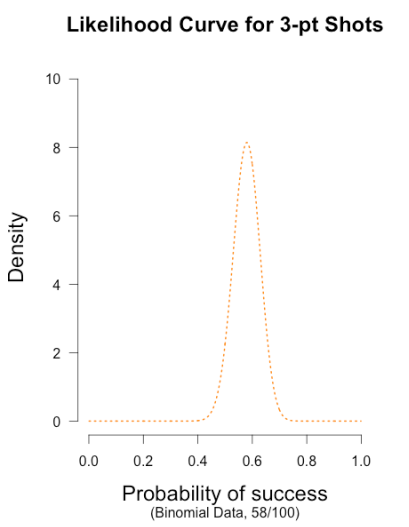
\includegraphics[width=0.4\textwidth]{pic/p05c03-snip05.png}
    \caption{Likelihood for 3-pt Shots}
    \label{fig:p05c03-snip05}
\end{figure*}

\FloatBarrier


\subsection{The prior}

Now the part that people often make a fuss about: choosing the prior. There are a few ways to choose a prior. Since I am using a binomial likelihood, I'll be using a conjugate beta prior. A beta prior has two shape parameters that determine what it looks like, and is denoted Beta($\alpha$, $\beta$). I like to think of priors in terms of what kind of information they represent. The shape parameters $\alpha$ and $\beta$ can be thought of as prior observations that I've made (or imagined).

Imagine my trusted friend caught the end of Brown's warm-up and saw her take two shots, making one and missing the other, and she tells me this information. This would mean I could reasonably use the common Beta(1, 1) prior, which represents a uniform density over [0, 1]. In other words, all possible values for Brown's shooting percentage are given equal weight before taking data into account, because the only thing I know about her ability is that both outcomes are possible\cite{LeeWagenmakers2005}.

Another common prior is called Jeffreys's prior, a Beta(1/2, 1/2) which forms a wide bowl shape. This prior would be recommended if you had extremely scarce information about Brown's ability. Is Brown so good that she makes nearly every shot, or is she so bad that she misses nearly every shot? This prior says that Brown's shooting rate is probably near the extremes, which may not necessarily reflect a reasonable belief for someone who is a college basketball player, but it has the benefit of having less influence on the posterior estimates than the uniform prior (since it is equal to 1 prior observation instead of 2). Jeffreys's prior is popular because it has some desirable properties, such as invariance under parameter transformation \cite{Jaynes2003}. So if instead of asking about Brown's shooting percentage I instead wanted to know her shooting percentage squared or cubed, Jeffreys's prior would remain the same shape while many other priors would drastically change shape.

Or perhaps I had another trusted friend who had arrived earlier and seen Brown take her final 13 shots in warm-up, and she saw 4 makes and 9 misses. Then I could use a Beta(4, 9) prior to characterize this prior information, which looks like a hump over .3 with density falling slowly as it moves outward in either direction. This prior has information equivalent to 13 shots, or roughly an extra 1/2 round of shooting.


\begin{figure}[h]
    \centering
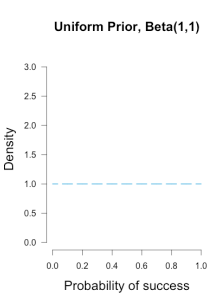
\includegraphics[width=0.3\textwidth]{pic/p05c03-snip06-1.png}
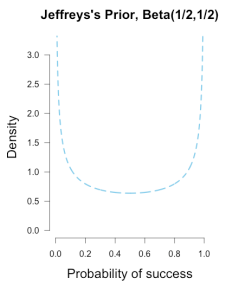
\includegraphics[width=0.3\textwidth]{pic/p05c03-snip06-2.png}
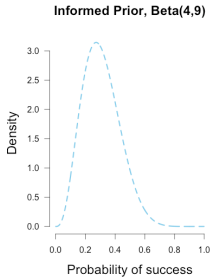
\includegraphics[width=0.3\textwidth]{pic/p05c03-snip06-3.png}
    \caption{Three different priors, or different Beta}
    \label{fig:p05c03-snip06}
\end{figure}

These are but three possible priors one could use. In your analysis you can use any prior you want, but if you want to be taken seriously you'd better give some justification for it. Bayesian inference allows many rules for prior construction.''This is my personal prior'' is a technically a valid reason, but if this is your only justification then your colleagues/reviewers/editors will probably not take your results seriously.

\FloatBarrier

\subsection{Updating the prior via the likelihood}

Now for the easiest part. In order to obtain a posterior, simply use Bayes's rule:

Posterior $\propto$ Likelihood $X$ Prior

The posterior is proportional to the likelihood multiplied by the prior. What's nice about working with conjugate distributions is that Bayesian updating really is as simple as basic algebra. We take the formula for the binomial likelihood, which from above is known to be:

Likelihood$=p^{x}(1-p)^{n-x}$

and then multiply it by the formula for the beta prior with $\alpha$ and $\beta$ shape parameters:

Prior$=p^{\alpha-1}(1-p)^{\beta-1}$ 

to obtain the following formula for the posterior:

Posterior $=p^{x}(1-p)^{n-x} p^{\alpha-1}(1-p)^{\beta-1}$

With a little bit of algebra knowledge, you'll know that multiplying together terms with the same base means the exponents can be added together. So the posterior formula can be rewritten as:

Posterior $=p^{x} p^{\alpha-1}(1-p)^{n-x}(1-p)^{\beta-1}$

and then by adding the exponents together the formula simplifies to:

Posterior $=p^{\alpha-1+x}(1-p)^{\beta-1+n-x}$

and it's that simple! Take the prior, add the successes and failures to the different exponents, and voila. The distributional notation is even simpler. Take the prior, Beta($\alpha$, $\beta$), and add the successes from the data, $x$, to $\alpha$ and the failures, $n – x$, to $\beta$, and there's your posterior, Beta($\alpha+x$, $\beta+n-x$).

Remember from the previous that likelihoods don't care about what order the data arrive in, it always results in the same curve. This property of likelihoods is carried over to posterior updating. The formulas above serve as another illustration of this fact. It doesn't matter if you add a string of six single data points, 1+1+1+1+1+1+1 or a batch of +6 data points; the posterior formula in either case ends up with 6 additional points in the exponents.

\subsection{Looking at some posteriors}

Back to Brown's shooting data. She had four rounds of shooting so I'll treat each round as a batch of new data. Her results for each round were: 13/25, 12/25, 14/25, 19/25. I'll show how the different priors are updated with each batch of data. A neat thing about Bayesian updating is that after batch 1 is added to the initial prior, its posterior is used as the prior for the next batch of data. And as the formulas above indicate, the order or frequency of additions doesn't make a difference on the final posterior. I'll verify this at the end of the post.

In the following plots, the prior is shown in blue (as above), the likelihood in orange (as above), and the resulting posteriors after Brown's first 13/25 makes in purple.


\begin{figure}[h]
    \centering
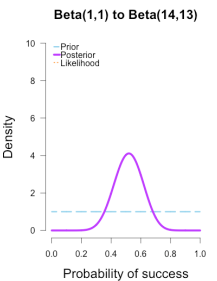
\includegraphics[width=0.3\textwidth]{pic/p05c03-snip07-1.png}
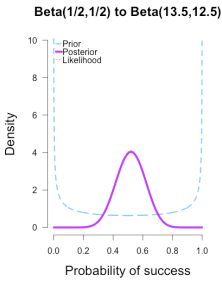
\includegraphics[width=0.3\textwidth]{pic/p05c03-snip07-2.png}
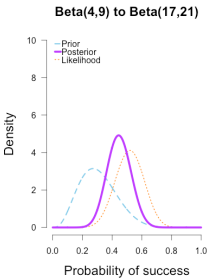
\includegraphics[width=0.3\textwidth]{pic/p05c03-snip07-3.png}
    \caption{Priors, likelihood and posteriors}
    \label{fig:p05c03-snip07}
\end{figure}

\FloatBarrier

In the first and second plot the likelihood is nearly invisible because the posterior sits right on top of it. When the prior has only 1 or 2 data points worth of information, it has essentially no impact on the posterior shape\footnote{There is a tendency to call any priors that have very little impact on the posterior ``non-informative'', but, as I mentioned in the section on determining priors, uniform priors that seem non-informative in one context can become highly informative with parameter transformation \cite{MuZhuLu2004}. Jeffreys's prior was derived precisely with that in mind, so it carries little information no matter what transformation is applied.} . The third plot shows how the posterior splits the difference between the likelihood and the informed prior based on the relative quantity of information in each.

The posteriors obtained from the uniform and Jeffreys's priors suggest the best guess for Brown's shooting percentage is around 50\%, whereas the posterior obtained from the informed prior suggests it is around 40\%. No surprise here since the informed prior represents another 1/2 round of shots where Brown performed poorly, which shifts the posterior towards lower values. But all three posteriors are still quite broad, and the breadth of the curves can be thought to represent the uncertainty in my estimates. More data $\rightarrow$ tighter curves $\rightarrow$ less uncertainty.

Now I'll add the second round performance as a new likelihood (12/25 makes), and I'll take the posteriors from the first round of updating as new priors for the second round of updating. So the purple posteriors from the plots above are now blue priors, the likelihood is orange again, and the new posteriors are purple.


\begin{figure}[h]
    \centering
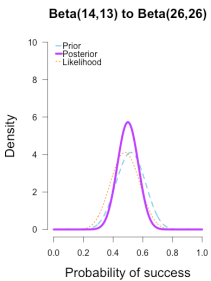
\includegraphics[width=0.3\textwidth]{pic/p05c03-snip08-1.png}
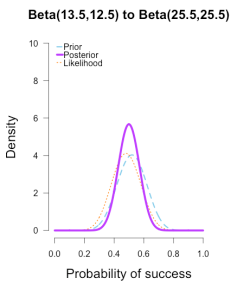
\includegraphics[width=0.3\textwidth]{pic/p05c03-snip08-2.png}
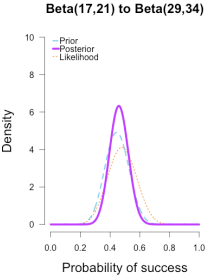
\includegraphics[width=0.3\textwidth]{pic/p05c03-snip08-3.png}
    \caption{Priors, likelihood and posteriors}
    \label{fig:p05c03-snip08}
\end{figure}


The left two plots look nearly identical, which should be no surprise since their posteriors were essentially equivalent after only 1 round of data updates. The third plot shows a posterior still slightly shifted to the left of the others, but it is much more in line with them than before. All three posteriors are getting narrower as more data is added.

The last two rounds of updating are shown below, again with posteriors from the previous round taken as priors for the next round. At this point they've all converged to very similar posteriors that are much narrower, translating to less uncertainty in my estimates.

\FloatBarrier


\begin{figure}[h]
    \centering
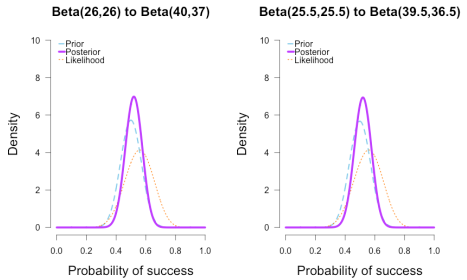
\includegraphics[width=0.6\textwidth]{pic/p05c03-snip09.png}
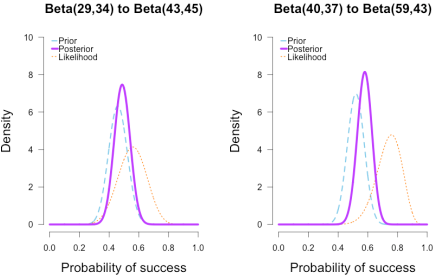
\includegraphics[width=0.6\textwidth]{pic/p05c03-snip10.png}
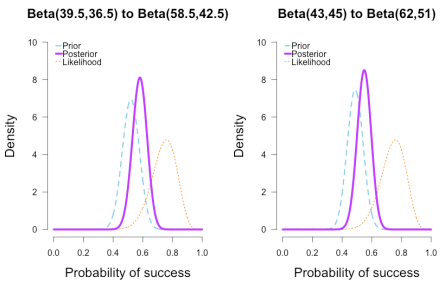
\includegraphics[width=0.6\textwidth]{pic/p05c03-snip11.png}
    \caption{Priors, likelihood and posteriors}
    \label{fig:p05c03-snip09}
\end{figure}

These posterior distributions look pretty similar now! Just as an illustration, I'll show what happens when I update the initial priors with all of the data at once.


\begin{figure}[h]
    \centering
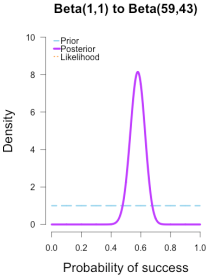
\includegraphics[width=0.3\textwidth]{pic/p05c03-snip12-1.png}
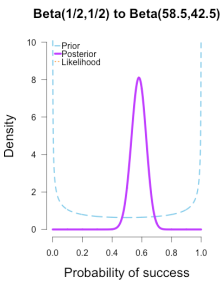
\includegraphics[width=0.3\textwidth]{pic/p05c03-snip12-2.png}
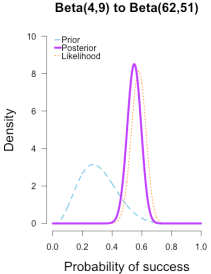
\includegraphics[width=0.3\textwidth]{pic/p05c03-snip12-3.png}
    \caption{Priors, likelihood and posteriors}
    \label{fig:p05c03-snip12}
\end{figure}

\FloatBarrier


As the formulas predict, the posteriors after one big batch of data are identical to those obtained by repeatedly adding multiple smaller batches of data. It's also a little easier to see the discrepancies between the final posteriors in this illustration because the likelihood curve acts as a visual anchor. The uniform and Jeffreys's priors result in posteriors that essentially fall right on top of the likelihood, whereas the informed prior results in a posterior that is very slightly shifted to the left of the likelihood.

My takeaway from these posteriors is that Cassandra Brown has a pretty damn good 3-point shot! In a future post I'll explain how to use this method of updating to make inferences using Bayes factors. It's called the Savage-Dickey density method, and I think it's incredibly intuitive and easy to use.
Notes:

\begin{lstlisting}
shotData<- c(1, 0, 0, 0, 1, 0, 1, 0, 1, 0, 0, 0, 1, 1, 1, 0, 1, 0, 1, 1, 1, 0, 0, 1, 1, 0, 0,
             1, 1, 1, 0, 0, 1, 1, 0, 0, 0, 1, 1, 1, 0, 0, 0, 0, 1, 1, 0, 1, 1, 0, 1, 0, 0, 1,
             0, 1, 0, 1, 1, 1, 0, 1, 0, 1, 0, 0, 1, 1, 0, 1, 0, 0, 1, 1, 1, 1, 1, 1, 1, 1, 1,
             1, 1, 1, 0, 0, 1, 1, 0, 0, 1, 1, 1, 0, 1, 1, 1, 1, 1, 0)

#figure 1 from blog, likelihood curve for 58/100 shots

x = seq(.001, .999, .001) ##Set up for creating the distributions
y2 = dbeta(x, 1 + 58, 1 + 42) # data for likelihood curve, plotted as the posterior from a beta(1,1)

plot(x, y2, xlim=c(0,1), ylim=c(0, 1.25 * max(y2,1.6)), type = "l", ylab= "Density", lty = 3,
     xlab= "Probability of success", las=1, main="Likelihood Curve for 3-pt Shots", sub= "(Binomial Data, 58/100)",lwd=2,
     cex.lab=1.5, cex.main=1.5, col = "darkorange", axes=FALSE)
axis(1, at = seq(0,1,.2)) #adds custom x axis
axis(2, las=1) # custom y axis

## Function for plotting priors, likelihoods, and posteriors for binomial data
## Output consists of a plot and various statistics
## PS and PF determine the shape of the prior distribution.
## PS = prior success, PF = prior failure for beta dist. 
## PS = 1, PF = 1 corresponds to uniform(0,1) and is default. If left at default, posterior will be equivalent to likelihood
## k = number of observed successes in the data, n = total trials. If left at 0 only plots the prior dist.
## null = Is there a point-null hypothesis? null = NULL leaves it out of plots and calcs
## CI = Is there a relevant X% credibility interval? .95 is recommended and standard

plot.beta <- function(PS = 1, PF = 1, k = 0, n = 0, null = NULL, CI = NULL, ymax = "auto", main = NULL) {
        
        x = seq(.001, .999, .001) ##Set up for creating the distributions
        y1 = dbeta(x, PS, PF) # data for prior curve
        y3 = dbeta(x, PS + k, PF + n - k) # data for posterior curve
        y2 = dbeta(x, 1 + k, 1 + n - k) # data for likelihood curve, plotted as the posterior from a beta(1,1)
        
        if(is.numeric(ymax) == T){ ##you can specify the y-axis maximum
                y.max = ymax
        }        
        else(
                y.max = 1.25 * max(y1,y2,y3,1.6) ##or you can let it auto-select
        )
        
        if(is.character(main) == T){
                Title = main
        }
        else(
                Title = "Prior-to-Posterior Transformation with Binomial Data"
        )
        
        
        plot(x, y1, xlim=c(0,1), ylim=c(0, y.max), type = "l", ylab= "Density", lty = 2,
             xlab= "Probability of success", las=1, main= Title,lwd=3,
             cex.lab=1.5, cex.main=1.5, col = "skyblue", axes=FALSE)
        
        axis(1, at = seq(0,1,.2)) #adds custom x axis
        axis(2, las=1) # custom y axis
        
        
        
        if(n != 0){
                #if there is new data, plot likelihood and posterior
                lines(x, y2, type = "l", col = "darkorange", lwd = 2, lty = 3)
                lines(x, y3, type = "l", col = "darkorchid1", lwd = 5)
                legend("topleft", c("Prior", "Posterior", "Likelihood"), col = c("skyblue", "darkorchid1", "darkorange"), 
                       lty = c(2,1,3), lwd = c(3,5,2), bty = "n", y.intersp = .55, x.intersp = .1, seg.len=.7)
                
                ## adds null points on prior and posterior curve if null is specified and there is new data
                if(is.numeric(null) == T){
                        ## Adds points on the distributions at the null value if there is one and if there is new data
                        points(null, dbeta(null, PS, PF), pch = 21, bg = "blue", cex = 1.5)
                        points(null, dbeta(null, PS + k, PF + n - k), pch = 21, bg = "darkorchid", cex = 1.5)
                        abline(v=null, lty = 5, lwd = 1, col = "grey73")
                        ##lines(c(null,null),c(0,1.11*max(y1,y3,1.6))) other option for null line
                }
        }
        
        ##Specified CI% but no null? Calc and report only CI
        if(is.numeric(CI) == T && is.numeric(null) == F){
                CI.low <- qbeta((1-CI)/2, PS + k, PF + n - k)
                CI.high <- qbeta(1-(1-CI)/2, PS + k, PF + n - k)
                
                SEQlow<-seq(0, CI.low, .001)
                SEQhigh <- seq(CI.high, 1, .001)
                ##Adds shaded area for x% Posterior CIs
                cord.x <- c(0, SEQlow, CI.low) ##set up for shading
                cord.y <- c(0,dbeta(SEQlow,PS + k, PF + n - k),0) ##set up for shading
                polygon(cord.x,cord.y,col='orchid', lty= 3) ##shade left tail
                cord.xx <- c(CI.high, SEQhigh,1) 
                cord.yy <- c(0,dbeta(SEQhigh,PS + k, PF + n - k), 0)
                polygon(cord.xx,cord.yy,col='orchid', lty=3) ##shade right tail
                
                return( list( "Posterior CI lower" = round(CI.low,3), "Posterior CI upper" = round(CI.high,3)))
        }
        
        ##Specified null but not CI%? Calculate and report BF only 
        if(is.numeric(null) == T && is.numeric(CI) == F){
                null.H0 <- dbeta(null, PS, PF)
                null.H1 <- dbeta(null, PS + k, PF + n - k)
                CI.low <- qbeta((1-CI)/2, PS + k, PF + n - k)
                CI.high <- qbeta(1-(1-CI)/2, PS + k, PF + n - k)
                return( list("BF01 (in favor of H0)" = round(null.H1/null.H0,3), "BF10 (in favor of H1)" = round(null.H0/null.H1,3)
                ))
        }
        
        ##Specified both null and CI%? Calculate and report both
        if(is.numeric(null) == T && is.numeric(CI) == T){
                null.H0 <- dbeta(null, PS, PF)
                null.H1 <- dbeta(null, PS + k, PF + n - k)
                CI.low <- qbeta((1-CI)/2, PS + k, PF + n - k)
                CI.high <- qbeta(1-(1-CI)/2, PS + k, PF + n - k)
                
                SEQlow<-seq(0, CI.low, .001)
                SEQhigh <- seq(CI.high, 1, .001)
                ##Adds shaded area for x% Posterior CIs
                cord.x <- c(0, SEQlow, CI.low) ##set up for shading
                cord.y <- c(0,dbeta(SEQlow,PS + k, PF + n - k),0) ##set up for shading
                polygon(cord.x,cord.y,col='orchid', lty= 3) ##shade left tail
                cord.xx <- c(CI.high, SEQhigh,1) 
                cord.yy <- c(0,dbeta(SEQhigh,PS + k, PF + n - k), 0)
                polygon(cord.xx,cord.yy,col='orchid', lty=3) ##shade right tail
                
                return( list("BF01 (in favor of H0)" = round(null.H1/null.H0,3), "BF10 (in favor of H1)" = round(null.H0/null.H1,3),
                             "Posterior CI lower" = round(CI.low,3), "Posterior CI upper" = round(CI.high,3)))
        }
        
}

#plot dimensions (415,550) for the blog figures

#Initial Priors
plot.beta(1,1,ymax=3.2,main="Uniform Prior, Beta(1,1)")
plot.beta(.5,.5,ymax=3.2,main="Jeffreys's Prior, Beta(1/2,1/2)")
plot.beta(4,9,ymax=3.2,main="Informed Prior, Beta(4,9)")

#Posteriors after Round 1
plot.beta(1,1,13,25,main="Beta(1,1) to Beta(14,13)",ymax=10)
plot.beta(.5,.5,13,25,main="Beta(1/2,1/2) to Beta(13.5,12.5)",ymax=10)
plot.beta(4,9,13,25,main="Beta(4,9) to Beta(17,21)",ymax=10)

#Posteriors after Round 2
plot.beta(14,13,12,25,ymax=10,main="Beta(14,13) to Beta(26,26)")
plot.beta(13.5,12.5,12,25,ymax=10,main="Beta(13.5,12.5) to Beta(25.5,25.5)")
plot.beta(17,21,12,25,ymax=10,main="Beta(17,21) to Beta(29,34)")

#Posteriors after Round 3
plot.beta(26,26,14,25,ymax=10,main="Beta(26,26) to Beta(40,37)")
plot.beta(25.5,25.5,14,25,ymax=10,main="Beta(25.5,25.5) to Beta(39.5,36.5)")
plot.beta(29,34,14,25,ymax=10,main="Beta(29,34) to Beta(43,45)")

#Posteriors after Round 4
plot.beta(40,37,19,25,ymax=10,main="Beta(40,37) to Beta(59,43)")
plot.beta(39.5,36.5,19,25,ymax=10,main="Beta(39.5,36.5) to Beta(58.5,42.5)")
plot.beta(43,45,19,25,ymax=10,main="Beta(43,45) to Beta(62,51)")

#Initial Priors and final Posteriors after all rounds at once
plot.beta(1,1,58,100,ymax=10,main="Beta(1,1) to Beta(59,43)")
plot.beta(.5,.5,58,100,ymax=10,main="Beta(1/2,1/2) to Beta(58.5,42.5)")
plot.beta(4,9,58,100,ymax=10,main="Beta(4,9) to Beta(62,51)")
\end{lstlisting}

\section{Visualization of the Bayes Factor}
\label{sec:VisualizationoftheBayesFactor}



\section{Evidence vs. Conclusions}
\label{sec:Evidencevs.Conclusions}



\section{How to become a Bayesian in eight easy steps}
\label{sec:HowtobecomeaBayesianineighteasysteps}




